\documentclass[variant=courcework]{bsuir}

\faculty{компьютерного проектирования}
\departmentlong{инженерной психологии и эргономики}
\departmentshort{эргономики}
\manager{эргономики}
\worktitle{Создание сервиса поиска визуально схожих изображений в
неорганизованных коллекциях}
\workcode{БГУИР КР 1-58 01 01 002 ПЗ}
\titleright{Студент\\Руководитель}
\titleleft{Бородин А.Н.\\Кабариха В.А.}
\titlepageyear{2024}

\graphicspath{{./assets/}}

\begin{document}

\maketitle

\clearpage\makeappendixpdf*{Задание по курсовой работе}*{task}*

\tableofcontents

\chapter*{Введение}

В современном мире объемы данных, включая изображения, растут с каждым днем.
Однако, с ростом количества данных возникает проблема поиска и классификации
информации. Визуальный поиск изображений становится особенно актуальным,
поскольку он позволяет пользователям находить изображения на основе их
визуальных характеристик, не зависимо от их текстового описания или тегов.

Сравнение изображений -- это процесс анализа двух или более изображений для
определения различий между ними. Это может включать в себя сопоставление
визуального содержания, такого как формы, цвета и текстуры, а также
использование алгоритмов для выявления изменений или аномалий. Сравнение
изображений широко используется в различных областях, включая цифровую
фотографию, медицинскую визуализацию, спутниковую разведку и системы
безопасности.

Целью данной курсовой работы является создание сервиса поиска визуально схожих
изображений в неорганизованных коллекциях на основе их визуальных характеристик,
таких как цвет, форма, текстура и других, даже если у них нет каких"=либо
метаданных, будь то теги или описание, который должен реализовать эффективную
систему индексации и хранения изображений, чтобы обеспечить быстрый доступ к ним
в коллекции и пользовательский интерфейс, который позволит пользователям
создавать выборки рассматриваемых файлов, следить за прогрессом сравнения и
просматривать результаты.

Данная работа будет включать в себя сравнительный анализ существующих решений,
оценочный выбор оптимальных инструментов для решения задачи, а также описание
разработанного сервиса. Будут представлены методы и алгоритмы, использованные
для сравнения изображений, описана система индексации и хранения данных, а также
представлен пользовательский интерфейс и результаты тестирования.

Ожидается, что результаты работы смогут применяться в реальных сценариях, где
требуется быстрый и точный поиск визуально схожих изображений в больших
коллекциях.

\chapter{Постановка задачи}

\section{Описание предметной области}

\subsection{Методики сравнения}
Визуальное сравнение изображений -- это процесс количественной оценки степени
визуального сходства между изображениями на основе извлекаемых из них
характеристик, с последующим ранжированием результатов. Можно выделить три
основных подхода к сравнению изображений: метрики структурного анализа,
хеширование изображений и использование машинного обучения.

\subsubsection{Метрики}
Метрика сходства -- это математическая абстракция для сравнения объектов,
присваивающая число, указывающее на степень родства между объектами указанной
пары \cite{ali2016survey}. Самый простой пример -- процент совпавших пикселей,
однако, существует множество более эффективных методов, различающихся по
сравниваемым признакам: цвет, текстура, форма и структура.

Метрики цвета количественно описывают распределение цветов и их статистические
характеристики в изображении. Чаще всего, речь о гистограммах. Гистограмма
изображения показывает частоту распределение пикселей различной интенсивности
показателя (цвет, освещенность и др.) \cite{ali2016survey}.

Метрики текстуры оценивают визуальные паттерны, структуру и неоднородности
поверхностей. Наиболее известны вейвлет"=преобразования. Вейвлет"=преобразование
одномерного сигнала состоит в его разложении по базису, сконструированному из
обладающей определенными свойствами солитоноподобной функции (вейвлета)
посредством масштабных изменений и переносов \cite{астафьева1996вейвлет}.

Метрики формы смотрят на геометрические и контурные особенности объектов.
Обычно, используются дескрипторы, такие как \textit{SIFT} (сравнение наборов
особых точек, найденных с помощью пирамиды гауссианов и ее разностей)
\cite{lowe2004distinctive}.

Наиболее популярны структурные метрики. Они позволяют оценить сходство
изображений по взаимосвязи между элементами. Каноничным примером алгоритма не
только структурного сравнения, но и визуального сравнения в целом считается,
имеющий десятки модификаций, \textit{SSIM} -- развитие методов \textit{RSNR} и
\textit{MSE}, с учетом специфики \textquote{восприятия ошибки}
\cite{wang2004image}.

\subsubsection{Хеширование}
Перцептивное хеширование -- отличается от метрики сходства наличием
промежуточного шага. Сравниваются не объекты, а их хеши. Операция сравнения
хешей проста и высокоэффективна, за счет чего можно значительно снизить
вычислительную нагрузку, если нужно сравнить эталон со множеством паттернов.
Вычисление всегда начинается с масштабирования изображения до маленького
размера, а затем проводится некоторое преобразование этой квадратной матрицы, в
зависимости от варианта алгоритма, за которым следует создание хеша из элементов
взятых в любом порядке. Для сравнения используют косинусное или Евклидово
расстояние или расстояние Хэмминга \cite{zauner2010implementation}.

Наиболее известны варианты основанные на дискретном косинусном преобразовании
(\textit{DCT}) для выделения низкочастотных компонентов (основной вариант,
Перцептивный хеш, \textit{pHash})\cite{zauner2010implementation}, на среднем
значении яркости (\textit{Average Hash}, \textit{aHash}), хеш радиального
отклонения (\textit{Radial Variance Hash}, \textit{vrHash}) и вейвлет"=функции
(\textit{Wavelet Hash}, \textit{wHash}) \cite{zauner2010implementation}.

\subsubsection{Машинное обучение}
Выделяется пять нейросетевых методов сравнения, которые позволяют извлекать и
сравнивать высокоуровневые визуальные признаки, что дает значительные
преимущества по сравнению с традиционными подходами. Они требуют несравнимо
больше аппаратных ресурсов чем метрики, однако гарантируют большую точность и
позволяют сравнивать смысловое содержание изображений: одинаковый ли объект (тип
объектов) на них изображен и на сколько они похожи.

Сети для извлечения дескрипторов обучаются извлекать компактные числовые
дескрипторы, описывающие визуальные характеристики изображений. Примером таких
сетей служит \textit{ResNet}\cite{simonyan2015deep}.

Сиамские нейронные сети состоят из двух или более идентичных подсетей, которые
обрабатывают несколько изображений параллельно; их обучают определять, являются
ли два изображения похожими или нет, на основе сравнения их внутренних
представлений \cite{koch2015siamese}.

Генеративные модели, например \textit{DCGAN}, могут сравнивать изображения на
основе их внутренних представлений \cite{radford2015unsupervised}.

Сети с контрастивным обучением используют методы контрастивного обучения для
различения похожих и непохожих изображений путем сравнения их внутренних
признаков, подобные \textit{SimCLR} \cite{DBLP:journals/corr/abs-2002-05709}.

Сети для семантической сегментации, такие как \textit{U-Net}, сравнивают
структуры и содержания на основе сегментированных областей
\cite{10.1007/978-3-319-24574-4_28}.

\subsection{Область применения}
Другой стороной предметной области является область применения. Сравнение
изображений находит широкое применение в различных сферах деятельности и
позволяет решать широкий спектр практических задач, связанных с анализом,
мониторингом и интерпретацией визуальной информации.

\subsubsection{Безопасность}
Одной из ключевых областей применения визуального сравнения изображений является
обеспечение безопасности и проведение наблюдения. Данная технология используется
для обнаружения изменений на охраняемых объектах, идентификации людей и
транспортных средств, мониторинга критической инфраструктуры, а также для
анализа видеонаблюдения в реальном времени с целью выявления аномалий и
подозрительной активности.

\subsubsection{Медицина}
В медицинской сфере визуальное сравнение изображений играет важную роль в
отслеживании прогрессирования или регрессии заболеваний, выявлении ранних
признаков патологий, оценке эффективности лечения, а также в автоматизированном
скрининге и диагностике на основе сравнения с базами данных типичных патологий.

\subsubsection{Промышленность}
Промышленность и производство также широко используют технологию визуального
сравнения изображений для контроля качества продукции, мониторинга
производственных процессов, отслеживания износа и повреждений оборудования, а
также для контроля качества упаковки и маркировки.

\subsubsection{Применение в быту}
Сравнение изображений применяется и в быту. Пользователи ищут по изображениям
именования заинтересовавших их предметов и желаемых товаров, местоположения
локаций и имена людей, изображенных на фотографиях, названия фильмов, передач и
сериалов по кадрам из них.

\subsubsection{Авторское право}
Кроме того, визуальное сравнение изображений находит применение в сфере
интеллектуальной собственности и авторского права. Эта технология используется
для поиска дубликатов и похожих изображений в больших базах данных,
классификации и каталогизации коллекций изображений, отслеживания использования
защищенных изображений в Интернете и выявления случаев плагиата.

\section{Сравнительный анализ}

\subsection{odiff}

\textit{odiff} -- консольная программа для сранения изображений. Она написана на
языке \textit{OCalm} и имеет привязку для использования в роли асинхронной
функции в \textit{nodejs}. Первый параметр вызова -- путь к эталонному
изображению, второй -- путь к изображению"=паттерну, с которым проводится
сравнение, а третий -- путь для записи результата сравнения. Само сравнение
проводится попиксельно и указывает красным цветом несовпадения. С заверения
разработчиков, программа в 6 быстрее ближайших конкурентов: \textit{pixelmatch}
и \textit{imagemagick compare} \cite{about-odiff}. Результаты работы изображены
на рисунке \ref{img:odiff}.

\makefigure{odiff}{
    \begin{subfigure}{.33\textwidth}
        \centering
        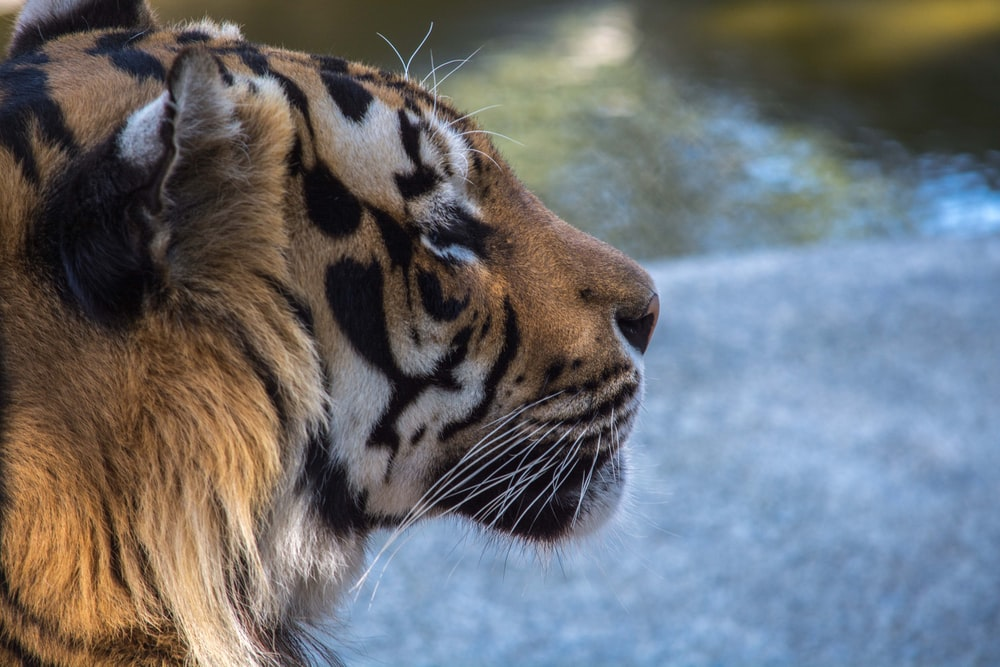
\includegraphics[width=.95\linewidth]{odiff1.jpg}
    \end{subfigure}%
    \begin{subfigure}{.33\textwidth}
        \centering
        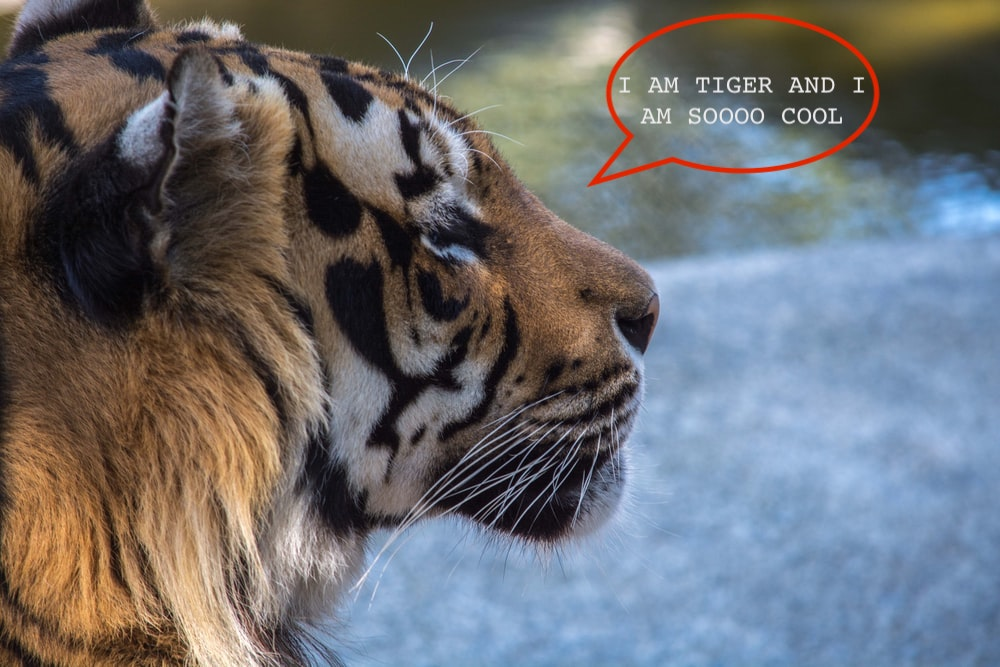
\includegraphics[width=.95\linewidth]{odiff2.jpg}
    \end{subfigure}%
    \begin{subfigure}{.33\textwidth}
        \centering
        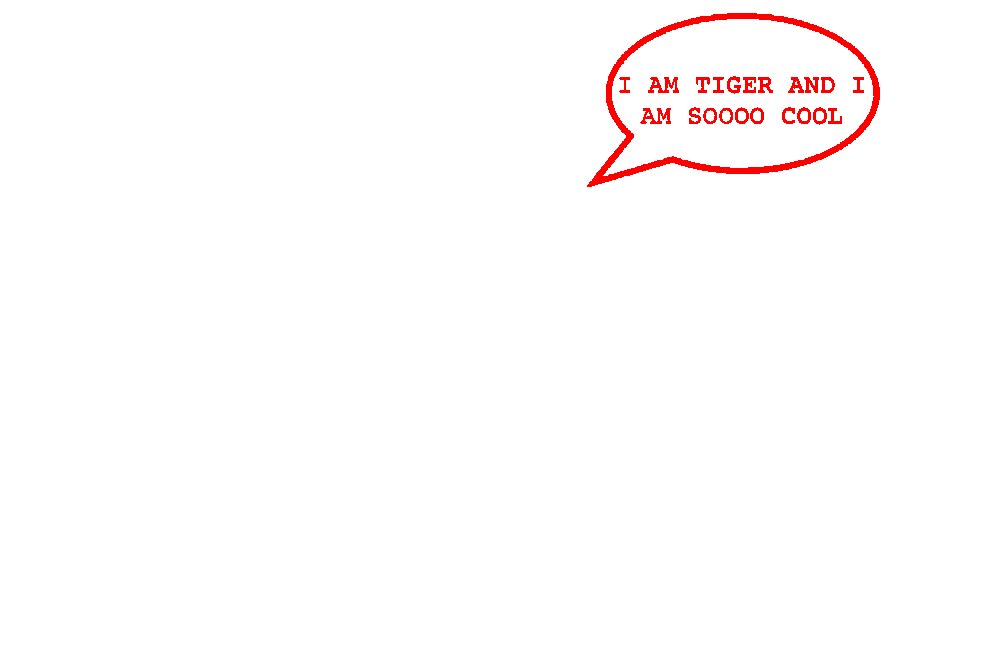
\includegraphics[width=.95\linewidth]{odiff3.png}
    \end{subfigure}
    \caption{Пример работы \textit{odiff}: эталон, паттерн, разница}
}

\subsection{ImageDeDup}
\textit{ImageDeDup} -- это библиотека на языке \textit{Python}, предназначенная
для поиска и удаления дублирующихся изображений. Она расчитана исключительно на
работу с изображениями и может быть встроена в другие программы или
использоваться непосредственно в роли утилиты в \textit{REPL}"=оболочке
\cite{about-imagededup}.

Библиотека предлагает несколько методов сравнения:

\begin{itemize}
    \item Сверточные нейронные сети (\textit{CNN}) -- использование готовых моделей
          или собственных.
    \item Перцептивное хеширование (\textit{PHash})
    \item Хеширование разностей (\textit{DHash})
    \item Вейвлет"=хеширование (\textit{WHash})
    \item Хеширование по средним значениям разностей (\textit{AHash})
\end{itemize}

\textit{ImageDeDup}, в первую очередь, ориентирована на исследовательские нужды
и работу с нейронными сетями, например, с использованием библиотек
\textit{NumPy} и \textit{Jupyter}. По"=этому она предоставляет возможность
генерации совмещенных изображений для иллюстрации результатов сравнения.

Для практического использования библиотека требует определенных навыков
программирования на \textit{Python}, так как код для выбора исходных файлов и
определения удаляемых дубликатов необходимо писать самостоятельно. На рисунке
\ref{img:imagededup.png} показан пример применения библиотеки для составления
сравнительного изображения для некоторого изображения со всеми в указанном
каталоге.

\makeimage[Пример применения \textit{ImageDeDup}]{imagededup.png}

\subsection{Czkawka}
Изображенная на рисунке \ref{img:czkawka.png}, \textit{Czkawka} -- наследница
заброшенного с 2017 года проекта \textit{FSlint}. В отличии от оригинала на
\textit{Python2/GTK+2} и работающего только под линукс-системами, разработан на
\textit{Rust/GTK4} (альтернативный фронтенд написан на \textit{slint}) и
кроссплатформенна. Программа обеспечивает широкий спектр интрументов для
поддержания порядка в файловой системе: помимо дедубликации посредством
универсального хеширования, имеются отдельные обработчики фото, аудио и видео,
поиск пустых и временных файлов и каталогов, невалидных ссылок и имен, больших
файлов. Для сравнение изображений используется настраиваемый перцептивный хеш
\cite{about-czkawka}.

Параметры перцептивного хеша:

\begin{itemize}
    \item Алгоритм масштабирования изображения: Lanczos3, ближайший сосед,
          треугольный, гауссовский, алгоритм Катмалла"=Рома;
    \item Размер хеша: 8, 16, 32, 64;
    \item Тип хеша: одинарный, вертикальный, двойной градиентный, блочный,
          средний.
\end{itemize}

\makeimage[Интерфейс \textit{Czkawka}]{czkawka.png}

\section{Информационная база задачи}

\subsection{Сводка}
Единственная информация, которую сервис сравнения изображений может хранить
между сеансами -- его конфигурация и, если еспользуется хеширование, кеш,
включающий в себя путь к файлу, его хеш и дату последнего изменения или иные
метаданные, сигнализирующие об изменении файла для пересчета его хеш"=суммы.
Форматы файлов выбираются в зависимости от фреймворка и вкусов разработчика. В
данной работе -- \textit{csv}.

\subsection{Местоположение}
Местоположение файлов конфигурации в \textit{linux}: \textit{/etc} для
общесистемных файлов и каталог, хранимый в переменной
\textit{\$XDG\_CONFIG\_HOME} или \textit{\$HOME/.config}, если таковой не
определено, для пользовательских параметров \cite{xdg_base_directory_spec}.

Кеш, если его сохраненность между перезапусками системы не требуется,
традиционно хранится в каталоге \textit{/etc}, иначе в
\textit{\$XDG\_CACHE\_HOME} или \textit{\$HOME/.local/}, если такового не
определено \cite{xdg_base_directory_spec}.

\section{Функциональное назначение}

\subsection{Задача}
Главное назначение программы -- составление списков изображений на основании их
показателя сходства и его интерпретации с последующим экспортом или обработкой. 

\subsection{Загрузка изображений}
Программа должна поддерживать самые популярные форматы изображений:
\textit{JPEG}, \textit{PNG}, \textit{TIFF}, \textit{BMP} и другие.

\subsection{Просмотр списка}
Важной функцией является просмотр списка сравниваемых изображений. В нем должна
отображаться информация об изображении, такая как название, показатели схожести,
размер файла, формат, дата съемки или любые иные полезные для пользователя
метаданные.

\subsection{Фильтрация}
Важной функцией является поиска по изображениям и сортировка их списка по
метаданным, таким как название, описание, теги, дата съемки, дата сохранения,
местоположение.

\subsection{Сравнение изображений}
Ключевой функцией программ для сравнения изображений является возможность
открывать и отображать два или более изображения одновременно для визуального
сравнения.

\subsection{Экспортирование списка}
Для пользователя будет очень удобна возможность экспорта списка сравниваемых
файлов с указанием экспортируемых полей списка, формата и пути, по которому он
будет сохранен. Форматами могут служить: \textit{JSON}, \textit{YAML},
\textit{CSV} и другие. Также можно реализовать генерацию скриптов для выполнение
каких"=либо действий над списком. К примеру, удаление дубликатов с показателем
схожести выше 98 процентов.

\subsection{Поддерживаемые платформы}
Поддержка \textit{linux} как целевой платформы.

\vspace{\baselineskip}
\phantomheading[section]{Заключение}

В разделе была рассмотрена задача о сравнение изображений, причины потребности
их сравнивать, существующие методы и программные решения. Помимо этого,
проведено их сравнение и оценена потребность в межсессионном хранении
информации, был составлен перечень требуемого функционала.

\chapter{Проектирование задачи}

В данном разделе описывается алгоритм вычисления хеша радиального отклонения,
структура программы и выбор инструментов разработки.

\section{Алгоритм решения задачи}

\subsection{Масштабирование изображения}
Масштабирование -- опциональный шаг, призванный повысить скорость обработки
изображения за счет уменьшения его размеров.

\subsubsection{Коэффициенты масштабирования}
Далее вычисляются коэффициенты масштабирования для осей X и Y путем деления
новых размеров на соответствующие старые.

\subsubsection{Создание нового изображения}
Создается новое изображение с заданными целевыми размерами. Обычно, это квадрат
с длиной стороны 8, 16, 32, 64 или 128.

\subsubsection{Интерполяция}
Проводится интерполяция значений цвета для каждого пикселя нового изображения на
основе значений цвета пикселей исходного. Для хеша не существенно качество
результата проведенной интерполяции, поэтому используется самая быстрая
интерполяция -- ближайший сосед. При этом методе каждому пикселю нового
изображения присваивается значение цвета ближайшего пикселя исходного
изображения.

\subsection{Обесцвечивание}
Для каждого пикселя уменьшенного изображения вычисляется среднее значение
цветовых каналов и присваивается пикселю в новом изображении, созданном заранее
в размерах, равных размеру уменьшенного изображения с целью уменьшения
информационной нагрузки изображения.

\subsection{Размытие Гаусса}
Размытие Гаусса -- последний шаг предобработки изображения, проводимый, чтобы
уменьшить влияние шумов на результат вычисления хеша. Можно подразделить на
две стадии: создание ядра Гаусса и фильтрацию.

\subsubsection{Создание ядра Гаусса}

Ядро Гаусса представляет собой матрицу чисел размером  с плавающей точкой,
которые вычисляются по данной формуле: риориоиоь ь ьииормомпомпрмпрмрмрс

% \[\begin{array}{c}
%             x=i-\frac{s}{2},\label{eq:x} \\
%             y=j-\frac{s}{2},\label{eq:y} \\
%             \dfrac{e^{-\frac{x^2 + y^2}{2\sigma^2}}}{2\pi\sigma^2}.\label{eq:kernel}
%       \end{array}\]\\
% \begin{tabular}{r c l}
%       где $x$, $y$ & -- & Расстояние до центра по оси $Ox$ ($Oy$); \\
%       $i$, $j$     & -- & Текущее положение по оси $Oy$; ($Oy$);   \\
%       $s$          & -- & Длина стороны изображения;               \\
%       \(\sigma\)   & -- & стандартное отклонение.                  \\
% \end{tabular}

% Ядро Гаусса создается с заданным размером и стандартным отклонением с помощью
% метода get_gaussian_kernel.

\subsubsection{Фильтрация}

% Применяется фильтрация изображения с использованием созданного ядра Гаусса.

\subsection*{Разделение изображения на сектора}

% Изображение разделяется на несколько секторов с равным угловым шагом. Для
% каждого пикселя изображения определяется его сектор на основе угла, который он
% образует с центром изображения. Это позволяет учесть структурные особенности
% изображения.

\subsection*{Вычисление медиан и стандартных отклонений}

% Для каждого сектора изображения вычисляются медианы и стандартные отклонения
% яркости пикселей.

\subsection*{Составление хеша}

% На основе вычисленных медиан и стандартных отклонений секторов изображения
% формируется хеш, который представляет собой битовую последовательность,
% отражающую структурные особенности изображения.

% Вычисленный хеш преобразуется в целочисленное значение с помощью хеш-функции.

\subsection*{Сравнение хешей}

% Для сравнения двух хешей используется метрика сходства, основанная на сравнении
% значений хешей. Чем меньше различий между хешами, тем более похожи изображения.



\section{Логическое моделирование}
% 2.2 Описание модулей программы, каждый модуль описывается как самостоятельная
% единица, которая выполняет определённый набор функций в программе, нет
% ситуаций, когда модуль есть, чтобы есть. (Диаграмма классов)

\subsection{Файловый модуль}

Модуль, отвечающий за все взаимодействия с файловой системой

\subsection{Графический модуль}

\subsection{Модуль действий}



\section{Выбор и обоснование инструментов разработки}

\subsection{Язык программирования}
Сравнение изображений, как и любая операция над медиа"=данными, требует много
вычислений, что делает краеугольным вопрос оптимизации и производительности.
\textit{C++} заслуженно считается лидером по производительности, обычно
превосходя \textit{Rust} и не конкурируя с \textit{C}, будучи с ним совместимым
\cite{benchmarksgame}. \textit{Rust} более современный язык, стремящийся его
заменить, проигрывает в силу меньшей востребованности, из"=за чего, раз курсовая
работа выполняется в учебных целях, изучение \textit{C++} приоритетнее, а
\textit{C} и так его подмножество.

\subsection{Фреймворк}
Курсовая работа требует изучать новые технологии на ходу, из"=за чего, когда
зашла речь о выборе графического фреймворка \textit{GTK} был предпочтен более
сложному \textit{Qt}, реализующему свою вариацию \textit{STL}. В плане простоты
выигрывают \textit{WinForms} и \textit{wxWidgets}, однако, первый эксклюзивен
для \textit{Windows}"=систем, а второй, как и в случае с выбора языка,
проигрывает в популярности.

\subsection{Библиотеки}
В 2021 году, из"=за слишком сильной привязанности \textit{GTK} к \textit{GNOME},
было решено вынести ряд стандартных окон и форм в отдельную библиотеку,
названную \textit{Adwaita}, а в зависимости от того, используется ли она,
называться программы на \textit{GTK} \textit{GNOME}"= и
\textit{GTK}"=приложениями соответственно. В силу эстетической притягательности
форм, библиотека была подключена.

\subsection{Система сборки}
Для сборки проекта была использована комбинация \textit{Meson} и \textit{Nix}.
Первый -- рекомендованная разработчиками \textit{GTK} и \textit{GNOME}
современная декларативная система сборки, лучше адаптированная к \textit{GTK},
чем \textit{CMake} и в разы превосходящая слишком сложный, но малофункциональный
\textit{Autoconf}. Для установки зависимостей был использован \textit{nix},
пакетный менеджер с удобной функцией рабочих окружений в каталогах и
\textit{direnv} для их автоматической загрузки. Выбран, так как прост в
использовании, не засоряет систему дубликатами библиотек и не требует
дополнительной настройки для встраивания в цикл сборки, в отличии от
\textit{vcpkg}.

Для компиляции проекта использовался \textit{clang}, по причине того, что при
разработке использовались \textit{clangd} и \textit{clang-uml}, которые от него
зависят, тестирование проводилось на процессоре \textit{AMD}, из"=за чего от
выбора \textit{ICC} бы не было бы какого"=либо преимущества, а причин выбрать
его прямого конкурента, \textit{GCC}, кроме репутации последнего, не имелось.

\subsection{Рабочая среда}
Для разработки программы был выбран редактор \textit{Visual Studio Code} по
следующим причинам:

\begin{itemize}
      \item Большой опыт его применения;
      \item Поддержка всех вышеназванных технологий через расширения, такие как
            \textit{clangd}, \textit{direnv}, \textit{Meson};
      \item За счет расширений формируется среда не только разработки программы,
            но и верстки пояснительной записки. Ключевая причина, так как
            воссоздать ее в другом \textit{IDE} будет тяжело.
\end{itemize}

В экосистеме \textit{GTK4} существует несколько способов разработки графического
интерфейса: программирование вручную, использование \textit{XML}"=описания,
\textit{blueprint}"=файлов или \textit{RAD}. Большинство разработчиков
предпочитают избегать описания интерфейса непосредственно в коде, так как это
приводит к избыточности и усложняет понимание программы. Использование
Декларативных \textit{XML} и \textit{blueprint}, также имеют свои недостатки, в
частности, громоздкость и проблемы с поддержкой некоторых функций
соответственно.

По"=этому, для проектирования пользовательского интерфейса был выбран
\textit{Cambalache} -- \textit{RAD}"=среда, пришедшая на смену устаревшему
\textit{Glade} и поддерживающая \textit{GTK4}.


\chapter{Программная реализация}

\section{Физическая структура}

\subsection{src/assets}

\textit{src/assets} -- Каталог с ресурсами приложения.

\subsection{src/assets/logo}

\textit{src/assets/logo} -- Каталог с логотипами приложения.

\subsection{src/assets/logo/128x128.png}

\textit{src/assets/logo/128x128.png} -- Логотип приложения размером 128x128
пикселей.

\subsection{src/assets/logo/256x256.png}

\textit{src/assets/logo/256x256.png} -- Логотип приложения размером 256x256
пикселей.

\subsection{src/assets/logo/512x512.png}

\textit{src/assets/logo/512x512.png} -- Логотип приложения размером 512x512
пикселей.

\subsection{src/assets/logo/scalable.svg}

\textit{src/assets/logo/scalable.svg} -- Логотип приложения в векторном формате.

\subsection{src/assets/meson.build}

\textit{src/assets/meson.build} -- Файл сборки ресурсов.

\subsection{src/assets/template.desktop}

\textit{src/assets/template.desktop} -- Шаблон файла \textit{.desktop} для
создания ярлыка приложения.

\subsection{src/gresources.xml}

\textit{src/gresources.xml} -- Перечень ресурсов приложения для их загрузки в
приложении.

\subsection{src/tests}

\textit{src/tests} -- Каталог с модульными тестами.

\subsection{src/tests/meson.build}

\textit{src/tests/meson.build} -- Файл сборки модульных тестов.

\subsection{src/tests/main.cc}

\textit{src/tests/main.cc} -- Точка входа в модульные тесты.

\subsection{src/views}

\textit{src/views} -- Каталог с файлами пользовательского интерфейса.

\subsection{src/views/about.ui}

\textit{src/views/about.ui} -- Файл пользовательского интерфейса для окна
\textit{About}.

\subsection{src/views/application.ui}

\textit{src/views/application.ui} -- Файл пользовательского интерфейса для
главного окна приложения.

\subsection{src/views/popover.ui}

\textit{src/views/popover.ui} -- Файл пользовательского интерфейса для
всплывающего окна.

\subsection{src/views/preferences.ui}

\textit{src/views/preferences.ui} -- Файл пользовательского интерфейса для окна
настроек.

\subsection{src/views/project.cmb}

\textit{src/views/project.cmb} -- Файл проекта \textit{Cambalache}.

\subsection{src/main.cc}

\textit{src/main.cc} -- Точка входа в приложение. В нем инициализируются
\textit{GetText} и \textit{adwaita}, создается экземпляр
\textit{CW1::Application} и запускается само приложение.

\subsection{src/meson.build}

\textit{src/meson.build} -- Файл сборки приложения. В нем собирается
испольняемый файл, загружается \textit{GResource} и запускается сборка тестов и
ресурсов.

\subsection{src/rvhash.hh}

\textit{src/rvhash.hh} -- Объявление класса \textit{CW1::RVHash} для хеширования
(модуль хеширования).

\subsection{src/rvhash.cc}

\textit{src/rvhash.cc} -- Имплементация класса \textit{CW1::RVHash} для
хеширования (модуль хеширования).

\subsection{src/application.cc}

\textit{src/application.cc} -- Имплементация класса \textit{CW1::Application}
для инициализации приложения и для обработки опций командной строки (модуль
приложения).

\subsection{src/application.hh}

\textit{src/application.hh} -- Имплементация класса \textit{CW1::Application} для
инициализации приложения и для обработки опций командной строки (модуль
приложения).

\subsection{src/processor.hh}

\textit{src/processor.hh} -- Объявление абстрактных классов
\textit{CW1::Processor} для обхода файлов (модуль итерации) и
\textit{CW1::Processor::Formatter} для форматирования вывода (модуль действий).

\subsection{src/hashformatter.cc}

\textit{src/hashformatter.cc} -- Имплементация класса
\textit{CW1::HashFormatter}, расширяющего класс
\textit{CW1::Processor::Formatter}, для обхода файлов (модуль итерации).

\subsection{src/hashformatter.hh}

\textit{src/hashformatter.cc} -- Объявление класса
\textit{CW1::HashFormatter}, расширяющего класс
\textit{CW1::Processor::Formatter}, для форматирования вывода (модуль действий).

\subsection{src/hashprocessor.cc}

\textit{src/hashprocessor.cc} -- Имплементация класса
\textit{CW1::HashProcessor}, расширяющего класс \textit{CW1::Processor}, для
обхода файлов (модуль итерации).

\subsection{src/hashprocessor.hh}

\textit{src/hashprocessor.cc} -- Объявление класса \textit{CW1::HashProcessor},
расширяющего класс \textit{CW1::Processor}, для обхода файлов (модуль итерации).

\section{Описание разработанных модулей}

\subsection*{Модуль приложения}

\subsubsection{\textit{CW1::Application}}

\textit{CW1::Application} -- класс, наследуемый от \textit{Gtk::Application}. Он
олицетворяет собою сеанс приложения, запускается из \textit{main}.

Публичные методы класса:

\begin{itemize}
    \item \textit{Application} -- инициализация приложения, включение режима
          ручной обработки опций программы и объявления опций командной строки.
    \item \textit{create} -- статический метод, который создает новый экземпляр
          класса \textit{Application} и возвращает его в виде умного указателя
          \textit{Glib::RefPtr} (на самом деле, это \textit{std::shared\_ptr}).
          Создан по аналогии с оригинальным классом \textit{Gtk::Application}
          для унификации поведения.
\end{itemize}

Защищенные методы класса:

\begin{itemize}
    \item \textit{on\_command\_line} -- метод, вызываемый при консольном запуске
          программы. Он обрабатывает опции командной строки и, если требуется,
          выполняет методы.
    \item \textit{on\_activate} -- обработчик сигнала \textit{activate}
          приложения. Он выполняется только при запуске графической сессии.
\end{itemize}

Приватные поля класса:

\begin{itemize}
    \item \textit{optionsFilters} -- объект группы опций. Объединяет те, что
          связаный настройкой поведения хеш"=функции.
    \item \textit{side, bins, sectors, sigma, stdDeviationThreshold,
          medianThreshold, rvhash} -- хранят экземпляр \textit{rvhash} и его
          параметры (нельзя получить значение опции из группы, не присваивая ее
          полю класса).
\end{itemize}

\subsection*{Модуль хеширования}

\subsubsection{\textit{CW1::RVHash}}

\textit{CW1::RVHash} -- класс"=обертка, объединяющий в себе методы все методы
для вычисления хеша радиальной дисперсии (\textit{Radial Variance Hash}). Методы
полностью соответствуют шагам, описанным в разделе \ref{sec:2.1}. 

Публичные элементы класса:

\begin{itemize}
    \item \textit{hash} -- псевдоним типа \textit{uint64\_t}. Формат хеша.
    \item \textit{compute} -- Вычисляет типа \textit{hash} хеш переданного ему
          изображения в формате \textit{Gdk::PixBuf} из соответственной
          библиотеки.
    \item \textit{compare} -- сравнивает хеши и возвращает
          \textit{double}"=показатель сходства. При верной конфигурации хеша
          находится в диапазоне от 0 до 1 и аналогичен проценту шанса
          совпадения.
\end{itemize}

Защищенные методы класса:

\begin{itemize}
    \item \textit{on\_command\_line} -- метод, вызываемый при консольном запуске
          программы. Он обрабатывает опции командной строки и, если требуется,
          выполняет методы.
    \item \textit{on\_activate} -- обработчик сигнала \textit{activate}
          приложения. Он выполняется только при запуске графической сессии.
\end{itemize}

Приватные методы класса:

\begin{itemize}
    \item \textit{get\_scaled} -- возвращает изображение нового размера:
          квадрат, длина стороны которого равна \textit{size}.
    \item \textit{get\_grayscale} -- обесцвечивает изображение.
    \item \textit{get\_sector\_stats} --обертка для метода \textit{get\_median}
          и \textit{get\_stddeviation}, обрабатывающая нулевые значения.
    \item \textit{get\_median} -- возвращает медиану значений пикселей
          изображения.
    \item \textit{get\_stddeviation} -- возвращает стандартное отклонение
          значений пикселей изображения.
    \item \textit{get\_gaussian\_blur} -- возвращает изображение, размытое
          гауссовым фильтром.
    \item \textit{get\_gaussian\_kernel} -- возвращает ядро гауссова фильтра.
    \item \textit{get\_filtered} -- возвращает изображение, прошедшее фильтрацию
          по ядру.
\end{itemize}

Приватные поля, у каждого из которых есть свой сеттер:

\begin{itemize}
    \item \textit{size} -- длина стороны квадрата, в который преобразуется
          изображение.
    \item \textit{bins} -- интервалы, по аналогии с \textit{OpenCV}. Кажется,
          они нигде не используются.
    \item \textit{sectors} -- количество секторов.
    \item \textit{sigma} -- стандартное отклонение размытия по Гауссу.
    \item \textit{stdDeviationThreshold} -- пороговое значение стандартного
          отклонения.
    \item \textit{medianThreshold} -- порогое значение медианы.
\end{itemize}

\subsection*{Модуль итерации}

\subsubsection{\textit{CW1::Processor}}

\textit{CW1::Processor} -- абстрактный класс для обхода файловой системы и
вывода результатов, используя \textit{CW1::Processor::Formatter}. Тоже
использует внутри себя \textit{CW1::RVHash}, по"=этому дублирует весь набор
сеттеров и приватных полей параметров хеша.

Публичные элементы класса:

\begin{itemize}
    \item \textit{Table} -- псевдоним типа \textit{std::map<std::string,
          CW1::RVHash::hash>}. Таблица хешей.
    \item \textit{process\_filepaths} -- виртуальный метод, возвращает
          таблицу хешей.
    \item \textit{process\_file} -- виртуальный метож, который обрабатывает
          файл и добавляет хеш в таблицу хешей, передаваемую вторым аргументом.
    \item \textit{set\_recursive} -- сеттер рекурсивного режима.
    \item \textit{set\_rvhash} -- сеттер экземпляра \textit{CW1::RVHash}.
    \item \textit{set\_formatter} -- сеттер экземпляра
          \textit{CW1::Processor::Formatter}.
    \item \textit{to\_string} -- возвращает строку отфарматированную строку.
    \item \textit{is\_image\_file} -- проверяет, является ли файл изображением,
          поддерживаемым \textit{Gdk::PixBuf}, за счет попытки его создания.
\end{itemize}

\subsubsection{\textit{CW1::HashProcessor}}

\textit{CW1::HashProcessor} -- реализация абстрактного класса, правила обхода:
для каждого каталога, обходит его содержимое, каталоги внутри него, только если,
указан флаг \textit{recursive}. Проверяет все файлы, являются ли они
изображениями. В полученний таблице будут вектора с одним элементом -- хешем
этого файла.

Определяет виртуальные методы \textit{process\_filepaths} и
\textit{process\_file}. Добавляет защищеный метод \textit{process\_directory},
реализующий рекурсию.

\subsection*{Модуль действий}

\subsubsection*{\textit{CW1::Processor::Formatter}}

Определяет только публичный виртуальный метод \textit{format}, который принимает
таблицу хешей и поток вывода, в который он записывает результаты.

\subsubsection*{\textit{CW1::HashFormatter}}

Реализует вывод хешей в форме: \textquote{путь к файлу | хеш}. Вывод
отфарматирован так, что образуется цельтая вертикальная черта.

\vspace{\baselineskip}
\phantomheading[section]{Заключение}

В разделе были составлены перечни файлов и описаны разработанные модули. Для
каждого класса и метода дана краткая сводка, упомянуты детали реализации и
расписаны отношения между классами. Более точную информацию можно найти в
диаграмме классов, представленной в приложении \ref{sec:В}. Ее точность
гарантируется тем, что она была сгенерирована автоматически, используя утилиты
\textit{clang"=uml} и \textit{plantuml}.

\chapter{Тестирование}

Для тестирования программы был использован \textit{GLib Testing Framework},
являющийся частью \textit{GLib}, и \textit{Valgrind}, профилировщик системных
ресурсов. Сначала было проведено тестирование отдельных модулей программы, в
соответствии с 

В данном разделе курсовой работы будут рассмотрены различные аспекты
приведены Lib Testing Framework, оценку производительности с помощью профилировщиков
системных ресурсов, а также автоматизацию процесса тестирования с использованием
системы сборки Meson. Результаты тестирования будут тщательно документированы,
что позволит не только оценить текущее состояние приложения, но и определить
направления для его дальнейшего совершенствования.

\chapter{Применение программы}

\section{Руководство пользователя}

\subsection{Установка программы}

Поддерживается установка как пакета, используя пакетный менеджер \textit{nix},
дистрибутива \textit{NixOS}. Для этого необходимо выполнить следующие шаги:

\begin{enumerate}
    \item Получить код из репозитория на \textit{GitHub}:
          \url{https:://github.com/nadevko/bsuir-CW1}. Для этого выполнить
          команду: \texttt{git clone https://github.com/nadevko/bsuir-CW1}.
    \item Перейти в директорию с проектом: \texttt{cd bsuir-CW1}.
    \item Установить пакет: \texttt{nix-env -if .}. Он будет скомпилирован и добавлен
          в систему.
\end{enumerate}

Альтернативно, можно использовать \textit{nix-shell} для запуска программы в
изолированной среде. Для этого требуется иная завершающая команда:
\texttt{nix-\\build -E~'with import <nixpkgs> \{ \}; callPackage}.

\subsection{Справка по использованию}

Программе передается список файлов и каталогов

Программа поддерживает следующие опции командной строки:

\begin{itemize}
    \item \texttt{-h, --help} -- выводит справку по использованию;
    \item \texttt{--help-all} -- выводит все параметры справки;
    \item \texttt{--help-gapplication} -- показывает параметры
          \textit{GApplication};
    \item \texttt{--help-hash} -- выводит справку по параметрам хеширования;
    \item \texttt{-v, --version} -- выводит версию программы;
    \item \texttt{-r, --recursive} -- осматривает каталоги рекурсивко;
    \item \texttt{-m, --mode} -- определяет режим работы программы;
    \item \texttt{-e, --export} -- определяет формат вывода результата;
    \item \texttt{-s, --side} -- устанавливает длину строки;
    \item \texttt{-b, --bins} -- размер интервалов;
    \item \texttt{--sigma} -- стандартное отклонение размытия по Гауссу;
    \item \texttt{--deviation} -- значение стандартного отклонения;
    \item \texttt{--median} -- значение отклонения медианы.
\end{itemize}


\chapter*{Заключение}

\bibliography{lib}

\chapter[обязательное]{Исходный код программы}

\makelisting{../src/application.cc}[src/application.cc]
\makelisting{../src/application.hh}[src/application.hh]
\makelisting{../src/gresources.xml}[src/gresources.xml]
\makelisting{../src/hashformatter.cc}[src/hashformatter.cc]
\makelisting{../src/hashformatter.hh}[src/hashformatter.hh]
\makelisting{../src/hashprocessor.cc}[src/hashprocessor.cc]
\makelisting{../src/hashprocessor.hh}[src/hashprocessor.hh]
\makelisting{../src/main.cc}[src/main.cc]
\makelisting{../src/processor.hh}[src/processor.hh]
\makelisting{../src/rvhash.cc}[src/rvhash.cc]
\makelisting{../src/rvhash.hh}[src/rvhash.hh]

\makeappendixpdf*[справочное]{Схема алгоритма хеширования}{assets/algorithm}

% \makeappendix{обязательное}{Диаграмма вариантов использования}{}

% \makeappendix[обязательное]{Диаграмма деятельности}{}

% \makeappendix[справочное]{Схемы алгоритмов}{}

% \makeappendix[справочное]{Диаграмма классов}{}

\makeappendixpdf*{Ведомость документов}*{inventory}

\end{document}
